\documentclass[12pt]{article}
\usepackage{mathpazo}
\usepackage{graphicx}
\usepackage[explicit]{titlesec}
\usepackage{hyperref}
\usepackage[export]{adjustbox}
\usepackage{placeins}
\usepackage{subcaption}
\usepackage{import}
\usepackage[dvipsnames]{xcolor}
\usepackage{listings}
\usepackage{setspace}


\begin{document}
\onehalfspacing
%title page
\begin{center}
	{\huge {\textbf{Politecnico di Milano}}}
	 	\vspace{7mm}\\
	 	
 	 	
\includegraphics[scale=1.5]{Images/PolimiLogo.png}
	\end{center}

\begin{center}
	     \vspace{5mm}
		{\Large A.A 2019/2020} 
		\vspace{5mm}\\
		{\Large {\textbf{Requirements Analysis and Specifications Document}}}   
		 
		
\includegraphics[scale=1]{Images/LOGO.jpg}
    \end{center}
          
\begin{flushright}
         
	 	 
	 	{\huge {\Large \textbf{Authors:}}}
	 	 
	 	{Armenante Valerio}
	 	
	 	{Capaldo Marco}
	 	
	 	{Di Salvo Dario}
	\end{flushright}


%begin of contents

\newpage
\hrule
\hypersetup{hidelinks}\tableofcontents

\vspace{0.5mm}
\vspace{0.24mm}

\newpage

\section{Introduction}
\hrule
\vspace{8mm}
\subsection{Purpose}
\vspace{5mm}
       The aim of this document is to give an overview of the             requirements and specifications of the system to be developed. The goal of the document is to describe in detail all functional and non-functional requirements of the system, analysing the needs of the customer and explaining common use case scenarios. It will set a baseline for project planning and cost es- timation, giving a detailed insight to all stakeholders which include the SafeStreets Investors and engineers (present and future) involved in development, testing and maintenance. 

\subsection{Scope}
\vspace{5mm}
\subsubsection{Description of the given problem}
\vspace{2mm}
	
	\textbf{SafeStreets Basic Service}

\vspace{3mm}
The given problem is to allow users to notify traffic violations to authorities. More specifically, the notification process consists in the acquisition of pictures, date, time, location and type of reported violation inserted by user. The aim of SafeStreets basic service is to retrieve and store information from inputted data, completing it with suitable metadata.  In particular, when user sends pictures related to a traffic violations, SafeStreets is able to recognize license plate by means of an external algorithm. After that, SafeStreets dispatches the notification to the authority member, which is in an available status and is chosen according to the minimum distance between the notified traffic violation and authority member’s position. In the end, the assigned authority member will opportunely manage the received request. In addiction, users and authorities member, through a Mobile Application interface presenting different level of visibility to different roles, will be able to mine information that has been received, for example by highlighting the areas with the highest frequency of violations. This is going to be realized designing some algorithms able to generate statistics on the previously stored data. A user who approaches the mobile application for the first time has to complete a registration process, as well as an authority which approaches the dedicated website for the first time. In particular, an authority inserts all their authority member in SafeStreets database through a website’s form specifying their e-mail and unique code. In this way, each authority member have to do only an activation process, inserting their personal data and the assigned unique code.

\vspace{5mm}

\begin{flushleft}
\textbf{SafeStreets Advanced Function 1}
\end{flushleft}
\vspace{3mm}
The goal of this SafeStreets’ first advanced function is to improve more the security of cities through a cooperation with municipality. First of all SafeStreets retrieves information from municipality through an external service, then information are categorized (accidents, violations, etc.) and some statistics are generated. Then crossing information between resultant elaboration and already available SafeStreets data, the goal can be reached. More specifically, if traffic violations cardinality, related to an area, exceed a specified threshold, SafeStreets identifies the area as unsafe and suggests possible interventions to municipality. Obviously, the threshold is properly defined according to the characteristics of the city.

\newpage

\begin{flushleft}
\textbf{SafeStreets Advanced Function 2}
\end{flushleft}
\vspace{3mm}
The goal of this SafeStreets’ second advanced function is to provide correct information, related to traffic violations, to municipality(in particular local police). In this way, municipality can easily and correctly emits traffic tickets to the offenders. In order to ensure the correctness of information, SafeStreets implements an algorithm that recognize if a manipulation is occurred on uploaded data by users. Moreover, Safestreets builds some statistics regarding traffic tickets data such as a ranking of the most offenders, most common violations and the effectiveness of SafeStreets initiative.
\vspace{4mm}
\begin{center}
	
	 	\vspace{4mm}
	 	
 	 	\includegraphics[scale=0.75]{Images/Immagine.png}
 	 	\textbf{Table 1.1:} Wold and Machine table.
	\end{center}


\newpage


\subsubsection{Goals}
\vspace{5mm}
\begin{flushleft}
Here are summarized goals that must be achieved by SafeStreets:
\vspace{2mm}

\textbf{[G1]}: Users can be uniquely identified, thanks to the completion of the Registration Process.\vspace{1mm}

\textbf{[G2]}: Authorities can be uniquely identified, thanks to the completion of Registration Process.
\vspace{1mm}

\textbf{[G3]}: Authority members can be uniquely identified, thanks to the completion of Authentication Process.
\vspace{1mm}

\textbf{[G4]}: Allows users to notify authorities when traffic violations occur.
\vspace{1mm}

\textbf{[G5]}: Allows authority member to receive the notifications about traffic violations in order to increase the local security.
\vspace{1mm}

\textbf{[G6]}: Allows end users to mine information on traffic violations that has been received and build some statistics.
\vspace{1mm}

\textbf{[G7]}: Allows authorities to mine information on traffic violations that has been received and build some statistics.\vspace{1mm}

\textbf{[G8]}: Builds a cross information analysis between municipality’s data and itself data in order to improve reliability of the service and suggest to municipality possible interventions. \vspace{1mm}

\textbf{[G9]}: Allows municipality (in particular local police) to retrieve traffic violations in order to generate relative traffic tickets.\vspace{1mm}

\textbf{[G10]}: Builds statistics using information related to emitted traffic tickets.
\end{flushleft}
\vspace{5mm}
\subsection{Definition, Acronyms and Abbreviations}
\vspace{5mm}
\subsubsection{Definition}
\vspace{2mm}
\begin{flushleft}

\textbf{Customer:} It is used inside the document when a functionality is ref
erred to End Users, Authority and Authority members.
\vspace{2mm}

\textbf{Hardened Database Model:} hardening refers to providing various means of protection in a computer system. 

\end{flushleft}

\subsubsection{Acronyms}
\vspace{2mm}
\begin{flushleft}

\textbf{GPS} – Global Positioning System
\vspace{2mm}\\

\textbf{RASD} – Requirement Analysis and Specification Document 
\vspace{2mm}\\


\textbf{SS} - SafeStreets
\vspace{2mm}\\


\textbf{DB} - Database
\vspace{2mm}\\


\textbf{AI} - Artificial Intelligence
\vspace{2mm}\\

\textbf{AM} - Authority Member
\end{flushleft}

\newpage

\subsubsection{Abbreviations}
\vspace{2mm}
\begin{flushleft}

\textbf{[Gn]} – n-goal 
\vspace{2mm}\\
\textbf{[Dn]} – n-domain assumption 
\vspace{2mm}\\
\textbf{[Rn]} – n-functional requirement 
\vspace{2mm}\\

\end{flushleft}
\vspace{2mm}
\subsection{Reference Document}
\vspace{2mm}
\begin{itemize}
\item IEEE Std 830-1998: “IEEE Recommended Practice for Software Requirements Specifications”

\item Project description: “Assignments AA 2019-2020.pdf”
\item Alloy Language Reference : \url{https://alloytools.org/documentation.html}
\item UML Language Reference : \url{https://www.utdallas.edu˜chung/Fujitsu/UML_2.0/Rumbaugh--UML_2.0_Reference_CD.pdf}
\end{itemize}

\subsection{Overview}
\vspace{2mm}
\begin{enumerate}
\item \textbf{Introduction}: this section gives a general description of the software  and its characteristics.

\item \textbf{Overall Descripion}: this section gives a general description of the software  and its characteristics.

\item \textbf{3.	Specific Requirements}: this section gives a deep insight about the system’s main functionality, analyzing scenarios with their relative use-cases and includes requirements(functional and not). Event flows are model using sequence and state diagrams. 

\item \textbf{Formal analysis using Alloy}: this section provides an Alloy model in order to give a detailed description of SS. Alloy is a declarative language used for specifying models of system and software.


\end{enumerate}

%CHAPTER 2
\newpage

\section{Overall Description}
\hrule
\vspace{8mm}

\subsection{Product Perspective}
\vspace{5mm}

The whole system is going to be developed from scratch, according to the choices written in this document. The registration process is always costless. Moreover, access and utilization for End Users, Authority member and Authority is free. This important choice has been made because of SafeStreets aim is to improve the security related to traffic violations, not a reason for earning money. 

\subsubsection{External Functions}
\vspace{2mm}

FindOwnerPlate is an external service that given in input a number plate then returns the owner of the vehicle. This service is well-integrated with SS and it is used to make faster traffic tickets process. 
\subsection{Product Functions}
Starting from the assumption that all the goals written in the previous part will be offered as functionalities of our system, we’re going to precisely list all the technical functions that the product will offer after its realization. 

\newpage

\subsubsection{Data storing management}
\vspace{5mm}
A relational DB is made available as storage memory for the whole ecosystem, in which all personal and non personal information, together with Customers’ gathered data, will be saved. It is mandatory to store data in a way that both security measures for sensitive information as well as fast and reliable access possibilities are guaranteed. To reach [G1] and [G2], it is necessary to exploit all the facilities provided by the Hardened Database model. The aim is to prevent data loss, leakage, or unauthorized access. At the registration time of each Customer, a new tuple will be created into the respectively table. Each Customer tuple will be uniquely linked to the Customer who own it. To reach that, a unique identifier will be generated for every Customer, to ensure that the associated data will be correctly extractable from the DB without ambiguities. The identifier assignment and the DB scanning mechanism will be chosen to be as fast as possible, since the system is going to be built for efficiently managing a huge amount of customers. Sequential DB scanning approaches as well as progressive identifiers assignment algorithms will be ignored during the choice. Finally, to ensure that any kind of information related to traffic violations are not altered, an encryption mechanism is put in place.

\subsubsection{Data sharing management}
\vspace{2mm}
SafeStreets gives top priority to Customer’s privacy. No data and traffic violation notification access will be granted to other Users. When a user notifies a traffic violation to an authority member, this one will share some limited personal data such as unique code, name and surname. All traffic violations can be accessed by both authority and authority members and SafeStreets gives the possibility to filter traffic violations using specific criteria. Moreover, an authority member can access to a personal panel that shows past traffic violations managed by him. 

\subsubsection{Traffic violations handler}
\vspace{2mm}
After that an end user sends traffic violations using SafeStreets service, then they are forwarded to the nearest authority member using a specific handler. SafeStreets uses an external service (such as Google Maps) to calculate the time spent by each authority member, in that zone, to arrive in traffic violation position. Then SafeStreets handler selects the authority member that has the minimum arrival time and this is done because often minimum distance, inside city, does not imply faster reaction.

\subsubsection{Municipality collaboration service }
\vspace{2mm}
In order to ensure a correct collaboration with municipality, SafeStreets’ system administrator communicates to an employee of municipality how information must be sent. After that a protocol is chosen then SafeStreets is able to store all information inside its DB and uses a specific algorithm to cross information. Using that analysis, SS identifies unsafe areas and suggests some pre-set improvements to municipality through an e-mail. 
\subsubsection{RecognizePlate}
\vspace{2mm}
RecognizePlate is a well-built algorithm that permits to SafeStreets to recognize plate from pictures sent by end users. When a picture is received, then RecognizePlate uses advanced AI techniques to recognize plate in the image and returns to SafeStreets the number plate.  
\subsubsection{Traffic tickets handler}
\vspace{2mm}
When traffic notifications are sent to an authority member belonging to local police, SafeStreets using RecognizePlate and then FindOwnerPlate, explained before, is able to provide all useful information to make traffic tickets. Obviously, SafeStreets gives the possibility to discard a traffic notification in case it is considered a false notification.

\subsection{User characteristics}
\vspace{5mm}
\subsubsection{Actors}
\vspace{2mm}
\begin{itemize}
\item \textbf{Visitor}: a person which has not yet completed the Registration Process. The only thing which it is able to do is to start the registration process. 

\item \textbf{User}: a person using SafeStreets services which has completed the Registration Process. 

\item \textbf{Authority}: an employee of an institution who represents a specific station of the institution itself. 

\item \textbf{Authority member}: a recognized authority member. It uses SafeStreets to receive notification related to traffic violations.

\item \textbf{Municipality}: an employee of Municipality who have the task to manage the communication with SafeStreets.

\item \textbf{System Administrator}: a person in charge of keeping the system up to date, checking Authority policies and behaviors.

\item \textbf{Device}: a device used to transfer significant, and well-represented, world Data to the system such as pictures of traffic violations.
\end{itemize}


\subsection{Assumptions, dependencies and contraints}
\vspace{3mm}
\subsubsection{Domain assumptions}
\begin{flushleft}

[D1] - Authorities correctly insert address of reference station.
\vspace{2mm}

[D2] - Authorities must provide to its authority member the unique code.
\vspace{2mm}

[D3] - Devices used by end users are supposed to have a camera and an integrated and enabled GPS sensor.
\vspace{2mm}

[D4] - Sent position is assumed to be reliable and precise.
\vspace{2mm}

[D5] - System is supposed to be well integrated with reading plate algorithm that has been already designed and is correctly working.
\vspace{2mm}

[D6] - Each already uploaded notification of violation is every time correctly received and stored by the software system.
\vspace{2mm}

[D7] - Authority members specify correctly its availability status.
\vspace{2mm}

[D8] - The authority knows the local traffic laws and the related fines.
\vspace{2mm}

[D9] - Authority member that accept to provide an intervention must check the correctness of traffic violations notified and signals to Safe Streets.
\vspace{2mm}

[D10] - Municipality can fulfill the improvements suggested by the software.
\vspace{2mm}

[D11] - Municipality service is well integrated with SafeStreets.
\vspace{2mm}

[D12] - Municipality has an active mail system and it is periodically checked by its own employee.
\vspace{2mm}

[D13] - External service(FindOwnerPlate) is well integrated with SafeStreets that permits to retrieve personal data of the vehicle’s owner.
\vspace{2mm}

[D14] – Every time an authority member starts working, has to
logs into the application and sets properly availability status.
\vspace{2mm}

\end{flushleft}
%%%% SECTION 3%%%%

\newpage
\section{Specific Requirements}
\hrule
\vspace{8mm}
\subsection{Exsternal Interface Requirements}
\vspace{2mm}
\subsubsection{Customer Interfaces}
\vspace{3mm}
%% formatting %%
		 
		 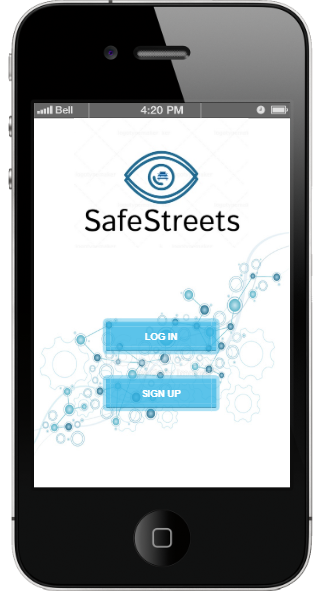
\includegraphics[scale=0.95]{MOCKUP/MOCKUPFIRST.png}                  \hfill 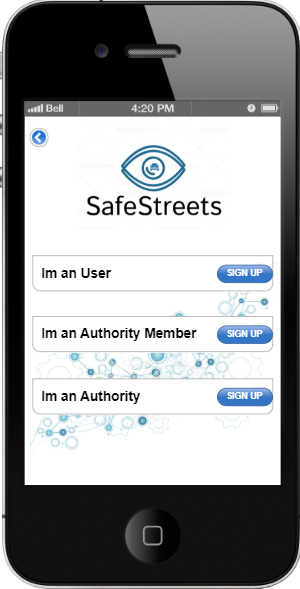
\includegraphics[scale=0.95]{MOCKUP/signup.png}
		 
		 \textbf{Figure 3.1:} SafeStreets home view.  \hfill \textbf{Figure 3.2:} SafeStreets Sign Up.
\newpage
 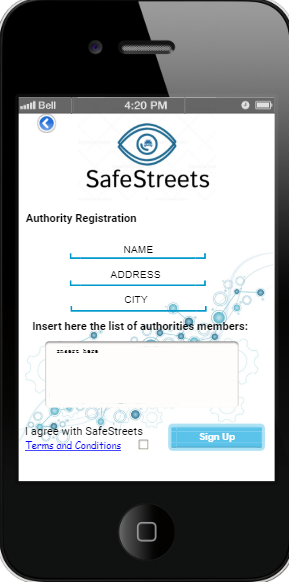
\includegraphics[scale=0.7]{MOCKUP/authreg.png}                  \hfill 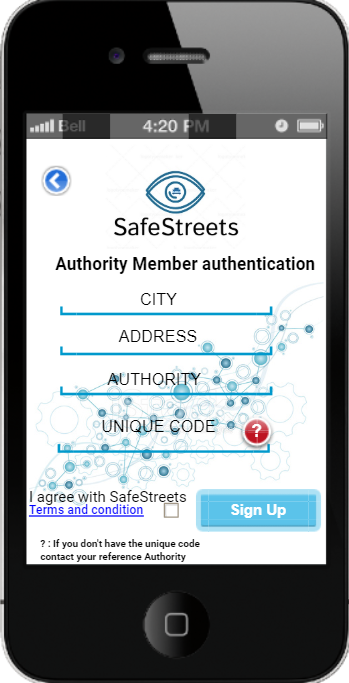
\includegraphics[scale=0.6]{MOCKUP/amreg.png}
		 
		 \textbf{Figure 3.3:} Authority registration   \hfill \textbf{Figure 3.4:} AM authentication.
		\begin{center}
  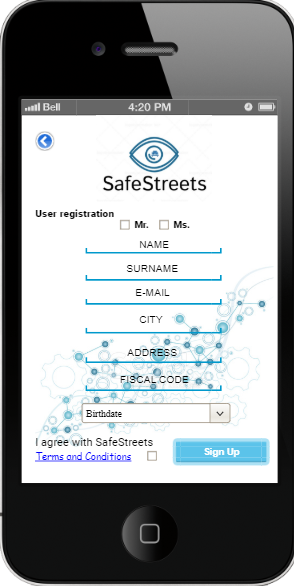
\includegraphics[scale=0.7]{MOCKUP/userreg.png}                  
  
		 \textbf{Figure 3.5:} User Registration.
	\end{center}


\newpage
 	 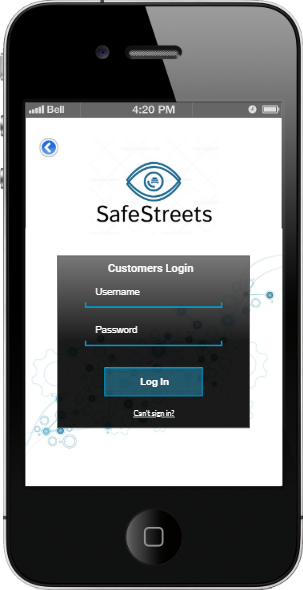
\includegraphics[scale=0.7]{MOCKUP/login.png}                  \hfill 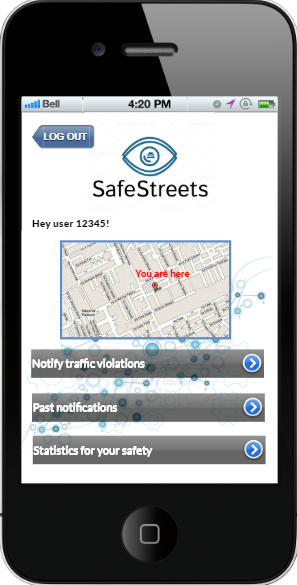
\includegraphics[scale=0.7]{MOCKUP/menuuser.png}
		 
		 \textbf{Figure 3.6:} Login view.  \hfill \textbf{Figure 3.7:} User Menu view.
		
  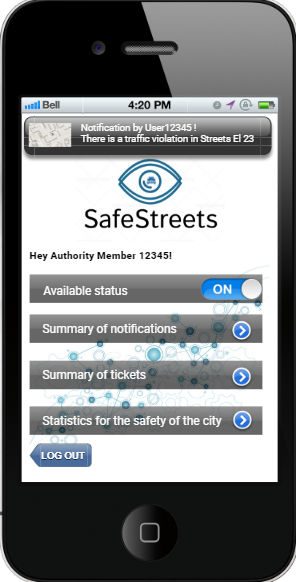
\includegraphics[scale=0.7]{MOCKUP/menuam.png}                  \hfill 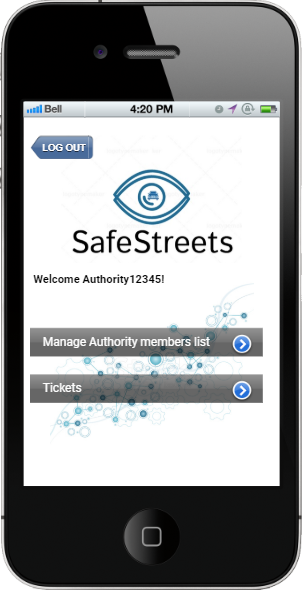
\includegraphics[scale=0.7]{MOCKUP/menua.png}
		 
		 \textbf{Figure 3.8:} Authority Member menu.  \hfill \textbf{Figure 3.9:} Authority menu.
		 

\newpage
 	 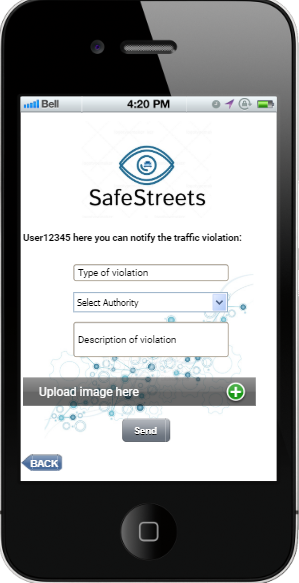
\includegraphics[scale=0.7]{MOCKUP/usernotification.png}                  \hfill 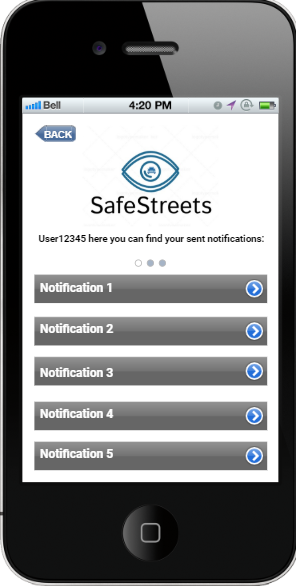
\includegraphics[scale=0.7]{MOCKUP/userpast.png}
		 
		 \textbf{Figure 3.10:} Notification's form user.  \hfill \textbf{Figure 3.11:} User notifications.
		
  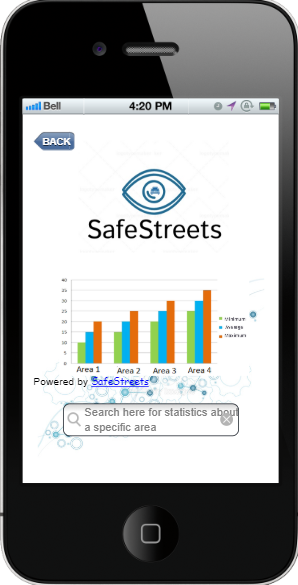
\includegraphics[scale=0.7]{MOCKUP/userstats.png}                  \hfill 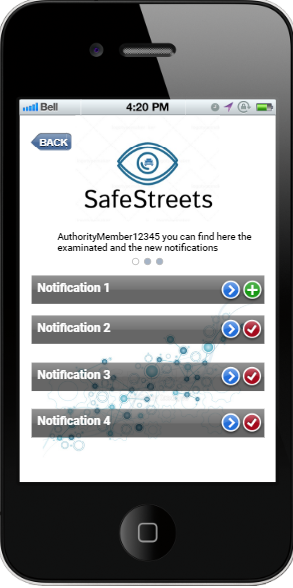
\includegraphics[scale=0.7]{MOCKUP/amnot.png}
		 
		 \textbf{Figure 3.12:} Statistics for user.  \hfill \textbf{Figure 3.13:}AM notifications.


\newpage
 	 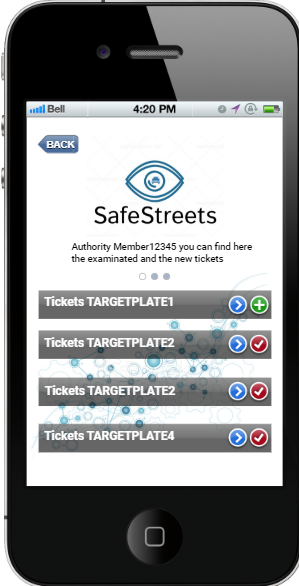
\includegraphics[scale=0.7]{MOCKUP/autmemtickets.png}                  \hfill 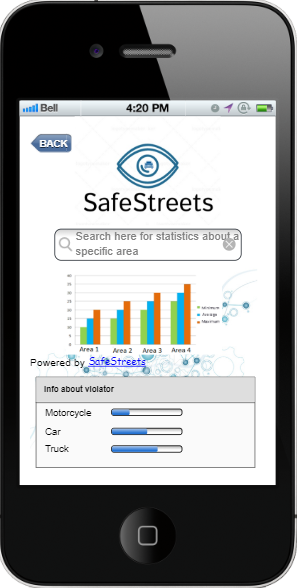
\includegraphics[scale=0.7]{MOCKUP/amstats.png}
		 
		 \textbf{Figure 3.14:} AM tickets menu   \hfill \textbf{Figure 3.15:} AM summary stats.
		
  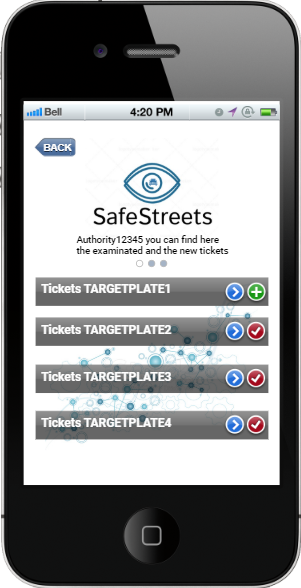
\includegraphics[scale=0.7]{MOCKUP/authtickets.png}                  \hfill 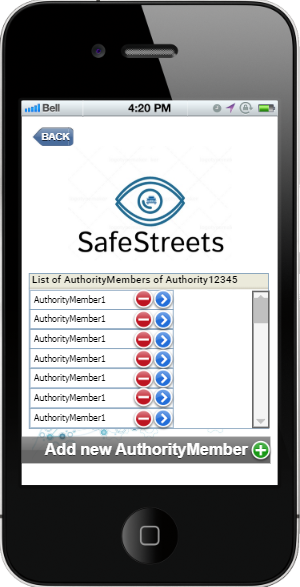
\includegraphics[scale=0.7]{MOCKUP/authmember.png}
		 
		 \textbf{Figure 3.16:} Authority tickets.  \hfill \textbf{Figure 3.17:} Authority members' list.

%% Hardware and Communication interface%% 

\subsubsection{Hardware and Communication Interfaces}
\vspace{5mm}
\begin{center}
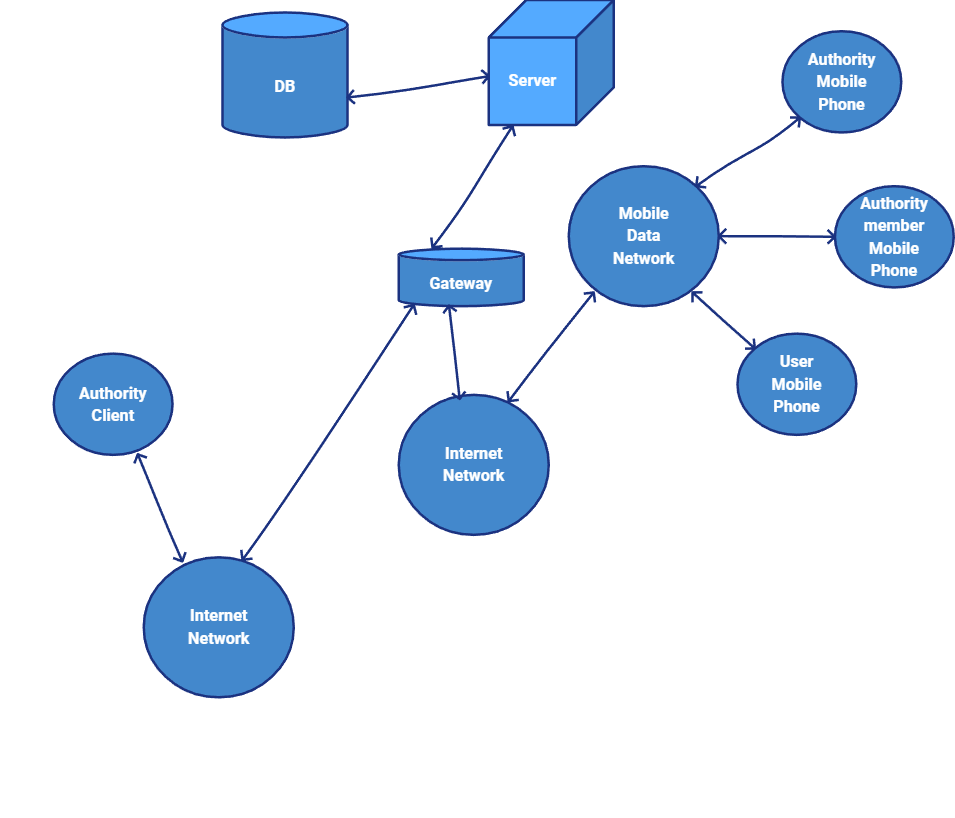
\includegraphics[scale=0.30]{communication/communication.png}                 

\textbf{Figure 3.16:} Communication architecture. 
\end{center}

\begin{center}
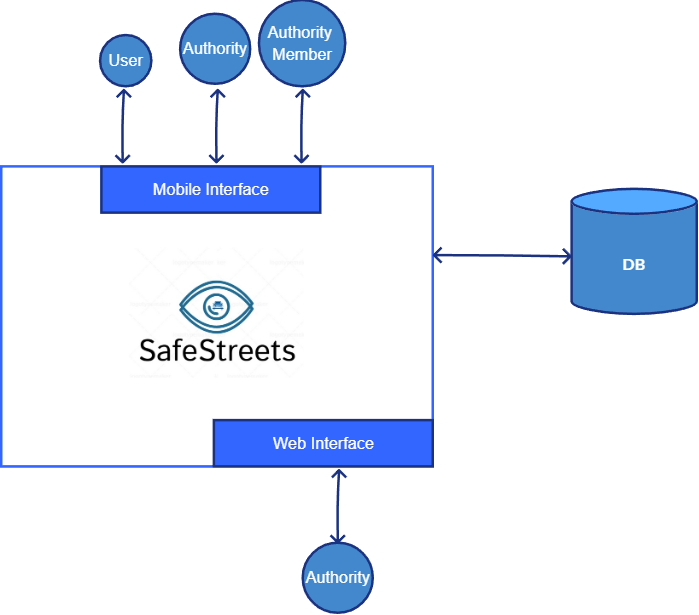
\includegraphics[scale=0.30]{communication/applicationdiagram.png}                 

\textbf{Figure 3.17:} Application diagram. 
\end{center}

\newpage

\subsection{Scenarios}
\subsubsection{Scenario 1}
\vspace{2mm}
Robert has a repair workshop in the heart of the city. Every morning someone parks in front of his garage’s workshop . So one of his employees advises him to install the SafeStreets application in his phone, so in this way he can notify to authorities the parking violation. Robert, after has downloaded the application, does the registration process and sends the traffic violation, filling the form and selecting the local police as authority. A local police authority member will arrive as soon as possible on the place, taking the relative judgment.


\subsubsection{Scenario 2}
\vspace{2mm}
Catherine booked a trip in a city thanks to her summer savings. On her journey, however, she realized that she needed help to understand the unsafe areas of the city. For this reason, Catherine asks in a police station whether or not there is a method of being able to have information on the streets that she have to avoid. The police reccomends her to download SafeStreets. After downloading and installing the application, Catherine proceeds to registration process as user. After that, she can interact with SafeStreets interface and access to the "Statistics" section, where she finds all the desired information about safeness in that city. 

\subsubsection{Scenario 3}
\vspace{2mm}

During everyday life, authorities have difficulties due to the high number of violations in metropolis. Directors of the various authority station (for example police, local police, etc.) gathered with the relative municipality to find some improvement that could help them to better manage all road violations. Thanks to a survey, the municipality finds SafeStreets to better manage the safeness of city streets. From this moment on, each authority joins to SafeStreets service, registering all its employees and each one of them will be able to log in to the application with a unique code provided to each of them. Finally, authority member can receive traffic violations by mean of notifications that are automatically managed by the system and showed to them through a panel.


\subsubsection{Scenario 4}
\vspace{2mm}
Local police station director noted that his employees have some difficulties in managing fines or traffic tickets in the best possible way. Sometimes, it may happen that fines are referred to wrong violations, or sometimes referred to the wrong car or other types of human errors. The local police director heard about the excellent impact that SafeStreets service have had in other cities, so he  decided to register his station, allowing users to access it. After downloading and installing the application, and registering all employees via forms, then all employees of the local police station are able to take in a correctly way the information about a traffic violations and generate the fines/tickets. 

\subsubsection{Scenario 5}
\vspace{2mm}
A municipality has to decide in which area of city organize a worldwide event that will be in 6 months. In order to accomplish this, the mayor contacts the authority, asking which are safe areas in according to collected data. The authorities are able to respond exactly to the request made by the municipality, since after registering on SafeStreets they can obtain information, thanks to the crossing of data analysis carried out by the application itself, on which areas are most secure in fast and exact way to the municipality. So now the municipality can decide thanks to given data where can manage the important event in the city.

\newpage

\subsection{Use cases diagrams}

\vspace{5mm}
\begin{center}
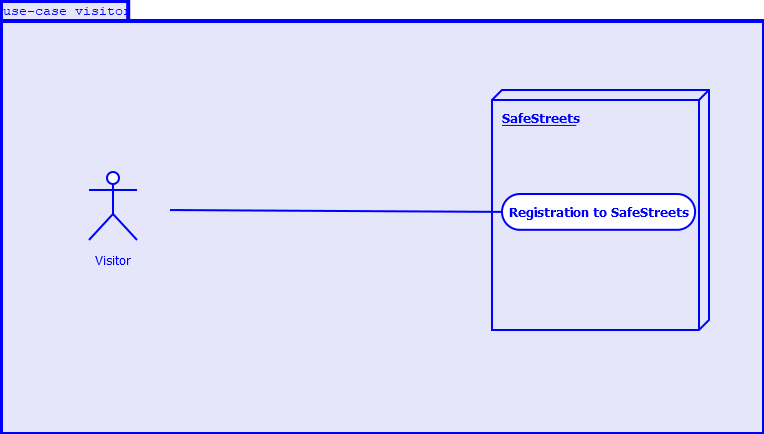
\includegraphics[scale=0.45]{Progettiuse-cases/Imgusecases/usecasevisitor.png}                 

\textbf{Figure 3.18:} Visitor use case. 
\end{center}

\begin{center}
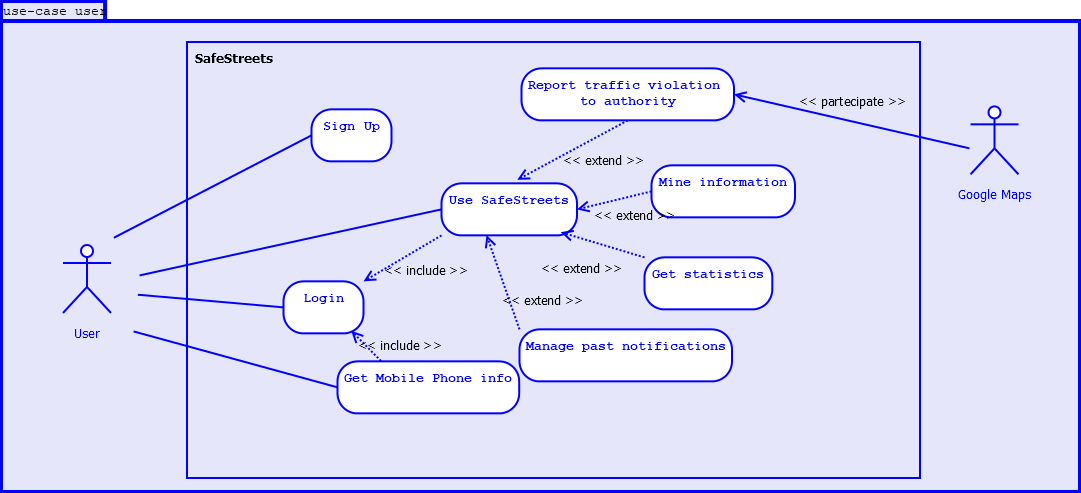
\includegraphics[scale=0.45]{Progettiuse-cases/Imgusecases/use-caseuser.png}                 

\textbf{Figure 3.19:} User use case. 
\end{center}

\newpage
\vspace{5mm}
\begin{center}
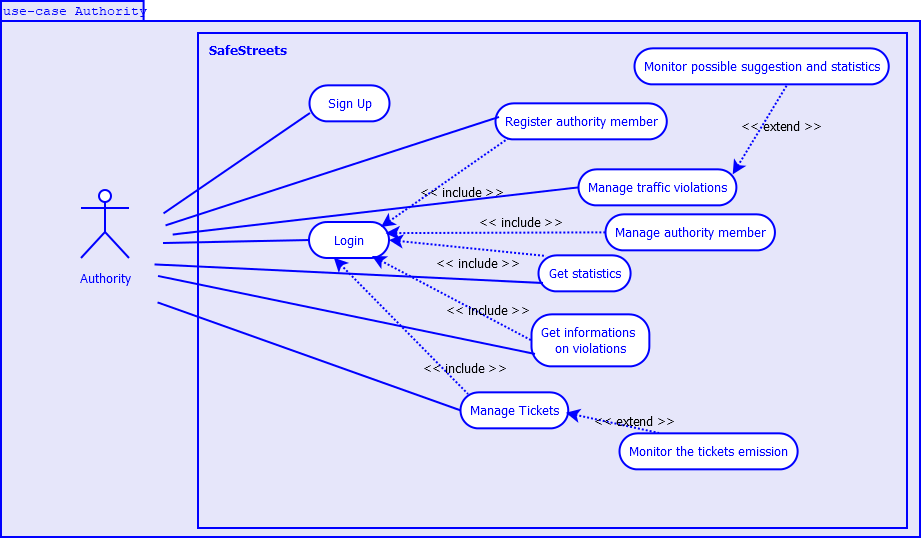
\includegraphics[scale=0.45]{Progettiuse-cases/Imgusecases/usecaseAuthority.png}                 

\textbf{Figure 3.18:} Authority use case. 
\end{center}

\begin{center}
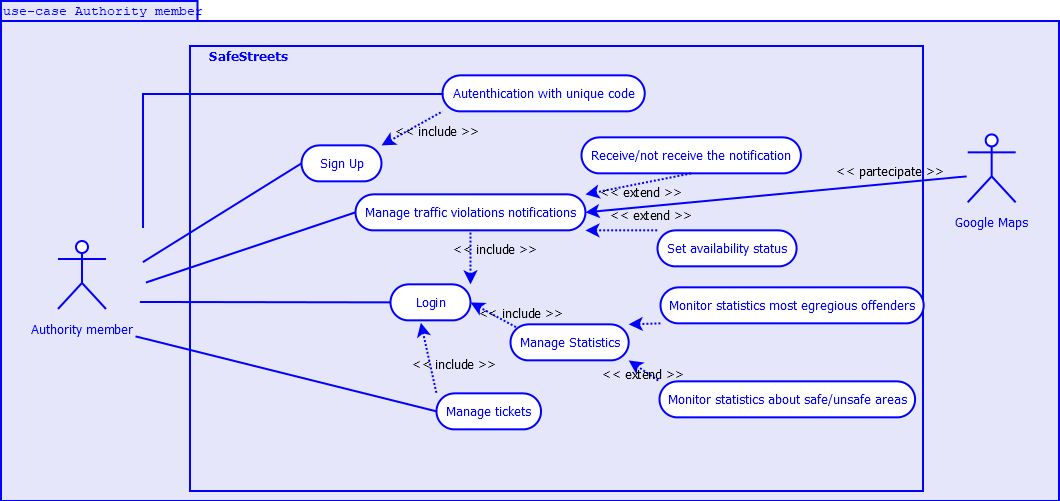
\includegraphics[scale=0.45]{Progettiuse-cases/Imgusecases/authmemb1.png}                 

\textbf{Figure 3.19:} Authority Member use case. 
\end{center}

\begin{center}
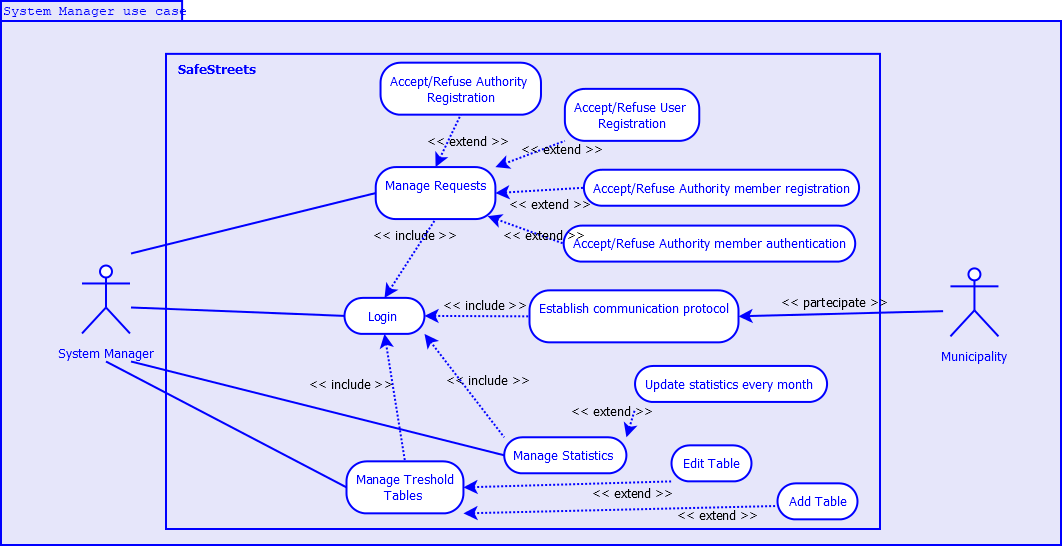
\includegraphics[scale=0.45]{Progettiuse-cases/Imgusecases/use-case-system.png}                  

\textbf{Figure 3.20:} System Manager use case. 
\end{center}

\newpage

%%%%FUNCTIONAL REQUIREMENTS%%%%
\subsection{Functional Requirements}
\vspace{5mm}

\subsubsection{SafeStreets Functional Requirements}
\vspace{2mm}%%GOAL1%%
\textbf{[G1]: Users can be uniquely identified, thanks to the completion of the Registration Process.}
\vspace{2mm}
\begin{flushleft}


[R1] -- Citizens must be able to begin the Registration Process into login page.
\vspace{2mm}

[R2] – During the Registration Process, Visitor have to be asked from the system for filling with his personal data (name, surname, address,birth date, gender, age, email, and fiscal code) a specific form.
\vspace{2mm}

[R3] – The system must reject the signup by a Visitor if the provided fiscal code is already associated to another existing account.
\vspace{2mm}

[R4] – The system must verify coherence between fiscal code inserted in the registration process form, and personal data provided by the user.
\vspace{2mm}

[R5] – The signup must include a completion process in order to verify the correctness of the user’s registration and enable the user to access to the software.
\vspace{2mm}

ciao
\vspace{2mm}

[R6] -- In order to complete Registration Process, the system will ask for an identity confirmation of the Visitor thanks to a code sent via email.
\end{flushleft}
%%%GOAL2%%%%
\vspace{4mm}
\textbf{[G2]: Authorities can be uniquely identified, thanks to the completion of Registration Process.}
\vspace{2mm}
\begin{flushleft}


[R7] -- Each authority, belonging to a town in which SafeStreets’ services are active, must be registered in order to lets its employee be notified by the users.
\vspace{2mm}

[R8] – After the Registration Process, Authority can manage the list of Authority Members adding or delete employees from the list.
\vspace{2mm}

[R9] – During the Registration Process, finalized by an Authority member, the system asks for the information about the physical information about the Authority, its formal force name (Police, Carabinieri, Local Police District), the address of reference station, an institutional mail addreass and a list of its employees (and for each of them provide name, surname, institutional email and an unique code).
\vspace{2mm}

[R10] – System when have the complete employees’ list, create an account for each of them.
\vspace{2mm}

[R11] – The system must reject the registration by an Authority if the provided set (formal name, address, city) is already associated to another existing one.
\vspace{2mm}

%%%GOAL 3%%%

\vspace{4mm}
\textbf{[G3]: Authority members can be uniquely identified, thanks to the completion of Activating Account Process.}
\vspace{2mm}

[R12] -- System must allow authority member to activate their own account providing the unique code that reference Authority Department has assigned to them.
\vspace{2mm}

[R13] – The sign up must include a completion process in order to verify the correctness of the user’s registration did by the Authority, and enable the Authority Member to access to the software.
\vspace{2mm}

[R14] – Software allows authority member to specify their availability status.
\vspace{2mm}

%%GOAL4%%%
\vspace{4mm}
\textbf{[G4]: Allows users to notify Authority Members when traffic violations occur.}
\vspace{2mm}

[R15] -- Users must provide their credentials, into the form of login page, to access to their personal area.
\vspace{2mm}

[R16] – If credentials do not match with the stored ones, the system must reject the request of login prompting an error.
\vspace{2mm}

[R17] – The mobile application must provide a section where the users can fill a form and upload images about the occurred traffic violations. In order to better organize force displacement user specifies to which Authority notify the violation.
\vspace{2mm}

[R18] –  The mobile application must provide a section where users can find all his past notifications.
\vspace{2mm}

[R19] – Allows end users to share the traffic violation’s position.
\vspace{2mm}

[R20] – Data and time are directly taken from end users’ device.
\vspace{2mm}

%%GOAL5%%
\vspace{4mm}
\textbf{[G5]: Allows authority member to receive the notifications about traffic violations in order to increase the local security.}
\vspace{2mm}

[R21] -- Authorities member must provide their credentials, into the form of login page, to access to their personal area.
\vspace{2mm}

[R22] – If credentials do not match with the stored ones, the system must reject the request of login prompting an error.
\vspace{2mm}

[R23] – Software system dispatches the notification about the incident to the nearest authority member, for which user requested an intervention. If the first authority member notified is busy, the notification will be passed to the next authority member always close to the incident.
\vspace{2mm}

[R24] –  Software permits to each authority member to specify their availability status.
\vspace{2mm}

[R25] – System must be able to recognize license plate from images.
\vspace{2mm}

[R26] – System must be able to recognize any possible kind of altered information contained in a traffic violation sent by a user.
\vspace{2mm}


%%GOAL6%%
\vspace{4mm}
\textbf{[G6]: Allows end users to mine information on traffic violations that has been received and build some statistics.}
\vspace{2mm}

[R22] -- Users must provide their credentials, into the form of login page, to access their personal view.
\vspace{2mm}

[R23] – Software system  shows statistics related to unsafe areas thanks to the highest number 
\vspace{2mm}

[R24] –  System shows to the end users the statistics in a specific section of the software.
\vspace{2mm}

[R25] –  Statistics must be updated each month.
\vspace{2mm}

%%GOAL7%%
\vspace{4mm}
\textbf{ [G7]: Allows authority members4 to mine information on traffic violations that has been received, and build some statistics.}
\vspace{2mm}

[R26] -- Software system show which kind of traffic violations occurs more frequently for each area.
\vspace{2mm}

[R27] – System shows the relate statistics in a specific section of the software.
\vspace{2mm}

[R28] – Software system is able to show statistics related to unsafe areas thanks to the highest number of traffic violations in that zone.
\vspace{2mm}

[R29] –  Statistics must be updated each month.
\vspace{2mm}

[R30] – Software system is able to show statistics related to vehicles that commit the most violations.
\vspace{2mm}

[R31] – Authority members must provide their credentials, into the form of login page, to access their personal view.
\vspace{2mm}

%%GOAL8%%
\vspace{4mm}
\textbf{ [G8]: Builds a cross information analysis between municipality’s data and its self data to improve reliability of the service and suggest to municipality possible interventions.}
\vspace{2mm}

[R32] -- Software system must be able to retrieve information from municipality service and generate their relative statistics.
\vspace{2mm}

[R33] – SafeStreets provides an algorithm able to cross information which derives from its own statistics and municipality’s statistics.
\vspace{2mm}

[R34] – Permits to suggest to municipality how to improve the security.
\vspace{2mm}

[R35] –  SafeStreets is able to communicate suggestion to the municipality through e-mail.
\vspace{2mm}

%%GOAL9%%
\vspace{4mm}
\textbf{ [G9]: Allows municipality (in particular local police) to retrieve traffic violations in order to generate relative traffic tickets.}
\vspace{2mm}

[R36] -- System has to avoid any possible kind of altered information contained in a traffic violation sent by a user.
\vspace{2mm}

[R37] – System must be able to recognize license plate from images.
\vspace{2mm}

[R38] – Provides personal data of the vehicle’s owner that committed an infraction to authorities, retrieved by an external service(FindOwnerPlate).
\vspace{2mm}

[R39] – SafeStreets is able to send all informations related to traffic violations to the nearest local police station that will handle ticket generation process assigning an authority member available in the zone.
\vspace{2mm}

[R40] – SafeStreets stores position of all local police centers in the city where SafeStreets works. 
\vspace{2mm}

%%GOAL10%%
\vspace{4mm}
\textbf{ [G10]: Builds statistics using information related to emitted traffic tickets.}
\vspace{2mm}

[R41] -- Provides personal data of the vehicle’s owner, who committed an infraction, to authorities retrieved by an external service.
\vspace{2mm}

[R42] – SafeStreets is able to store all infractions sent to local police station and generate their relative statistics by mean of an algorithm.
\vspace{2mm}

[R43] – SafeStreets provides to local police a ranking of the most offenders in their relative area.
\vspace{2mm}

[R44] –  SafeStreets provides to users the statistics concerning the improvement brought by SafeStreets initiative.
\vspace{2mm}



%%%%SEQUENCE DIAGRAMS NEW PAGE%%%
\end{flushleft}


%%%USE-CASE DESCRIPTION%%%

\subsubsection{Use case descriptions}
\vspace{5mm}
%% formatting %%
		 
		 \includegraphics[scale=0.9]{images/usecase1ok.png}                  
		 
		  \textbf{Table 3.1:} Registration Process – User (Citizen).

\newpage
	 
		 \includegraphics[scale=0.9]{images/usecase2.png}                  
		 
		  \textbf{Table 3.2:} Registration Process – Authorities.

\newpage

 \includegraphics[scale=0.9]{images/usecase3.png}                  
		 
		  \textbf{Table 3.3:} Activating Account Process – Authority Members.
		  
\newpage


 \includegraphics[scale=0.9]{images/usecase4.png}                  
		 
		  \textbf{Table 3.4:} Login Process – All.
		  
 \includegraphics[scale=0.9]{images/usecase5.png}                  
		 
		  \textbf{Table 3.5:} Notify Authority – User.
		  
\newpage

 \includegraphics[scale=0.9]{images/usecase6.png}                  
		 
		  \textbf{Table 3.6:} Authority Member handle violation report. 

\newpage

\begin{center}
\includegraphics[scale=0.90]{images/usecase8.png}                 

\textbf{Table 3.8:}Authority Members requests to visualize Statistics. 
\end{center}

\begin{center}
\includegraphics[scale=0.90]{images/usecase9.png}                 

\textbf{Table 3.9:} User requests to visualize progress of their past notifications. 
\end{center}

\newpage

\begin{center}
\includegraphics[scale=0.90]{images/usecase10.png}                 

\textbf{Table 3.10:}Authority Members requests to visualize their past handled notification.
\end{center}

\begin{center}
\includegraphics[scale=0.90]{images/usecase11ok.png}                 

\textbf{Table 3.11:} SafeStreets suggest same possible intervention to the Authority.
\end{center}

\newpage
 \includegraphics[scale=0.95]{images/usecase12ok.png}                  
		 
		  \textbf{Table 3.12:} Local police receives certified violations for  witch is possible to generate traffic tickets .

\newpage
 \includegraphics[scale=0.95]{images/usecase13.png}                  
		 
		  \textbf{Table 3.13:} Local police visualizes statistics regarding traffic tickets.
\vspace{5mm}
\subsection{ Performance Requirements}
\vspace{4mm}
\begin{flushleft}

[P1] – The system is designed to manage in an efficiently and effectively way the requests of a little-medium size city of about four hundred thousand population. In a first estimation, an average 75\% of contemporary users activity is expected.
\vspace{2mm}

[P2] – The system is designed to guarantee a response time less than 10 seconds between an user notification about a traffic violation and the succesful receipt and dispatching occurred between the agents closer to the streets’ violation.
\vspace{2mm}

[P3] – Starting from the System Manager, the system must guarantee the correcting update of every statics every month with a response time less than 30 seconds.
\vspace{2mm}

[P4] – Starting from the User notification to authorities, the system must guarantee a response time of less than 4 seconds for computing the accepting phase by the authorities member.
\newpage

\vspace{2mm}
[P5] – The system must guarantee an updating time of picture and infos in the form fill by the User about less than 3 seconds from the time the User updated the parameters and files.
\end{flushleft}


\subsection{Design Constraints}

\subsubsection{Standards compliance}

\subsubsection{Hardware limitations}
\vspace{3mm}\begin{itemize}
\item For the mobile app, an android 5+ or ios 10.1+ smartphone must be used.

\item One among WI-FI, 3G, 4G, 4G+ connection should be available in order to garantee the lowest latency.

\item A GPS sensor must be available on smartphone, and correctly face the SafeStreets data needs.

\end{itemize}

\subsection{Software System Attribute}
\vspace{2mm}
\subsubsection{Reliability}


\end{document}





